%% --------------------------------------------------------------
%%
%% I N T R O D U C T I O N
%%
%% --------------------------------------------------------------

\begin{frame}{}%%{Introduction}  %% ---------- Intro/motivation 

\begin{tikzpicture}[overlay,remember picture]

\uncover<1->{ % <-> |
    \node (t1) [anchor=center,scale=1,opacity=1] at ([shift={(-3.5cm,1.8cm)}]current page.center){
        \parbox{0.6\textwidth}{
            Binary neutron star (BNS) mergers are unique cosmic laboratories to study 
            \begin{itemize}
            \item theory of gravity in a strong field regime,
            \item matter at supranuclear densities,
            \item cosmic chemical evolution,%\nuc{} of the heaviest elements in the Universe,
            \item cosmology.%, using \ac{BNS} mergers as standard sirens
            \end{itemize}
    }};
}

\uncover<2->{ % <-> |
    \node (t1) [anchor=center,scale=1,opacity=1] at ([shift={(-3.5cm,-2.4cm)}]current page.center){
        \parbox{0.6\textwidth}{
            \GW{} 
            
            \begin{itemize}
            \item GWs, \GW{},
            \item Kilonova, \AT{}; bolometric light curves, spectra
            \item SGRB, \GRB{}; light curves, spectra, radio images 
            \item \textcolor{red}{\dots{}?}
            \end{itemize}

            %\red{Questions}: remnant's lifetime; ejecta mass/composition; sources of \rproc{} elements
    }};
}

\uncover<3->{ % <-> |
    \node (img1) [anchor=center,scale=1,opacity=1] at ([shift={(-2.0cm,-0.5cm)}]current page.center){
        \parbox{0.5\textwidth}{
            \textcolor{blue}{\texttt{arXiv}}: "968 results for all: GW170817" \\
    }};
}

\uncover<2->{ % <-> |
    \node (img1) [anchor=center,scale=1,opacity=1] at ([shift={(5.65cm,1.8cm)}]current page.center){
        \parbox{0.5\textwidth}{
            %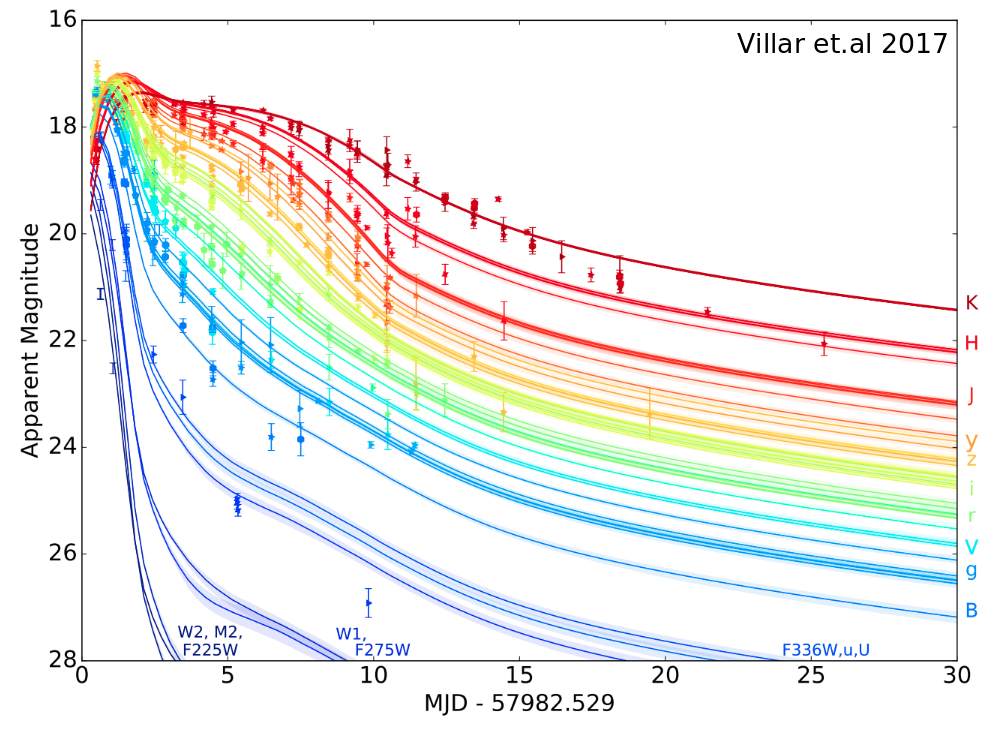
\includegraphics[height=3.8cm]{viller_mkn_model.png}
            \tiny{ Villar+17 \textcolor{gray}{arXiv:1710.11576} } \\
            \includegraphics[height=3.8cm]{Villar17_KNobs.pdf}
    }};
}
\uncover<2->{ % <-> |
    \node (img1) [anchor=center,scale=1,opacity=1] at ([shift={(5.5cm,-2.3cm)}]current page.center){
        \parbox{0.5\textwidth}{
%            \includegraphics[height=3.75cm]{Ghirlanda19_afterglow.pdf}
            \tiny{ Ghirlanda+19 \textcolor{gray}{arXiv:1808.00469} } \\
            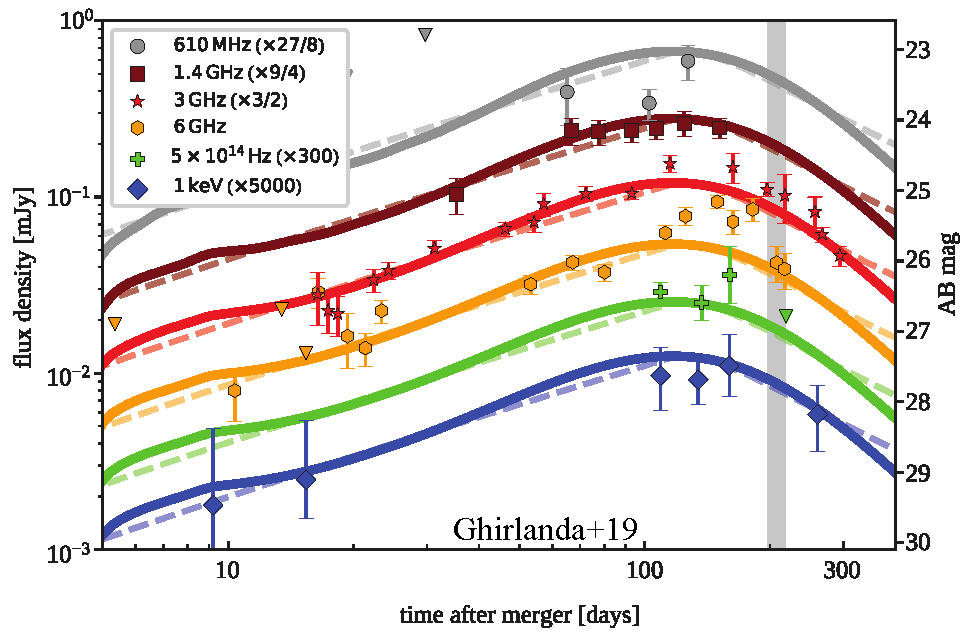
\includegraphics[height=3.75cm]{Ghirlanda19_GRB170817A.pdf}
            %\includegraphics[height=4.0cm]{Makhathini20_grb170817_afterglow.pdf}
    }};
}

\end{tikzpicture}
\end{frame}

\begin{frame}{}%%{Introduction}  %% ---------- Intro/motivation 

\begin{tikzpicture}[overlay,remember picture]

\uncover<1->{ % <-> |
    \node (t1) [anchor=center,scale=1,opacity=1] at ([shift={(-3.5cm,1.0cm)}]current page.center){
        \parbox{0.6\textwidth}{
            NR simulations + observations show 
            \begin{itemize}
            \item Tidal (dynamical) ejecta
            \item Shocked (dynamical) ejecta
            \item Post-merger winds (secular)
            \item GRB ejecta and cocoon
            \item Other?
            \end{itemize}
            \vspace{4mm}
            \dots{} BNS merger \textcolor{blue}{$\leftrightarrow$} ejecta \textcolor{red}{$\leftrightarrow$} EM signal \dots{} \\
    }};
    
}

\uncover<1->{ % <-> |
    \node (t1) [anchor=center,scale=1,opacity=1] at ([shift={(-3.5cm,-2.4cm)}]current page.center){
        \parbox{0.6\textwidth}{
            \begin{itemize}
            \item Kilonova: decay of $r$-process elements. Days-Weeks.
            \item Afterglow: synchrotron emission from shocked ISM. Weeks-Years. 
            \end{itemize}
    }};
}

\uncover<1-1>{ % <-> |
    \node (img1) [anchor=center,scale=1,opacity=1] at ([shift={(5.6cm,-0.5cm)}]current page.center){
        \parbox{0.5\textwidth}{
            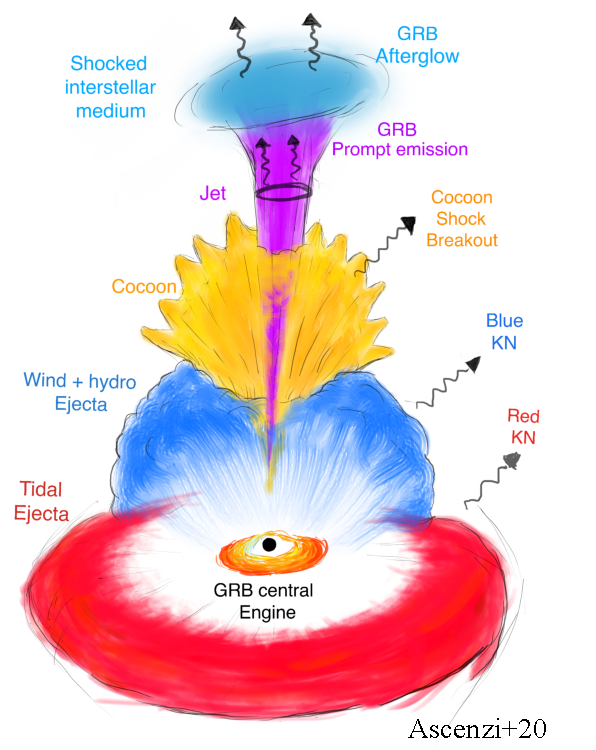
\includegraphics[height=7.5cm]{Ascenzi20_EjectaEMPicture.pdf}
            
            %\small{\textbf{Artist depiction of ejecta$^\text{\citep{Ascenzi:2020xqi}}$}}
    }};
}

\end{tikzpicture}
\end{frame}




%
%
%
%
%
%
%
%
%
%
%
%
%
%
%
%
%
%
%\begin{frame}{}%%{Introduction}  %% ---------- Intro/motivation 
%
%\begin{tikzpicture}[overlay,remember picture]
%
%\uncover<1->{ % <-> |
%    \node (t1) [anchor=center,scale=1,opacity=1] at ([shift={(-3.5cm,1.8cm)}]current page.center){
%        \parbox{0.6\textwidth}{
%            Binary neutron star (BNS) mergers are unique cosmic laboratories to study 
%            \begin{itemize}
%                \item theory of gravity in a strong field regime,
%                \item matter at supranuclear densities,
%                \item cosmic chemical evolution,%\nuc{} of the heaviest elements in the Universe,
%                \item cosmology.%, using \ac{BNS} mergers as standard sirens
%            \end{itemize}
%    }};
%}
%
%\uncover<1->{ % <-> |
%    \node (t1) [anchor=center,scale=1,opacity=1] at ([shift={(-3.5cm,-2.4cm)}]current page.center){
%        \parbox{0.6\textwidth}{
%            \GW{} 
%        
%            \begin{itemize}
%                \item \acp{GW}, \GW{},
%                \item \ac{kN}, \AT{}; (\rproc{} material decay),
%                \item \ac{SGRB}, \GRB{}; \textcolor{red}{\dots{}?},
%            \end{itemize}
%            
%            \textcolor{blue}{\texttt{arXiv}}: "968 results for all: GW170817" \\
%            %\red{Questions}: remnant's lifetime; ejecta mass/composition; sources of \rproc{} elements
%    }};
%}
%
%\uncover<1-1>{ % <-> |
%    \node (img1) [anchor=center,scale=1,opacity=1] at ([shift={(6.4cm,-0.5cm)}]current page.center){
%        \parbox{0.5\textwidth}{
%            \includegraphics[height=6.4cm]{jet_ascenci20.pdf}
%            
%            Artist depiction of ejecta$^\text{\citep{Ascenzi:2020xqi}}$
%    }};
%}
%
%\end{tikzpicture}
%\end{frame}
%
%%% --------------------------------------------------------------------------------
%
%\begin{frame}{}%%{Introduction}  %% ---------- Intro/motivation 
%
%\begin{tikzpicture}[overlay,remember picture]
%
%\uncover<1->{ % <-> |
%    \node (t1) [anchor=center,scale=1,opacity=1] at ([shift={(-3.5cm,1.5cm)}]current page.center){
%        \parbox{0.6\textwidth}{
%            Binary neutron star (BNS) mergers are unique cosmic laboratories to study 
%            \begin{itemize}
%            \item theory of gravity in a strong field regime,
%            \item matter at supranuclear densities,
%            \item cosmic chemical evolution,%\nuc{} of the heaviest elements in the Universe,
%            \item cosmology.%, using \ac{BNS} mergers as standard sirens
%            \end{itemize}
%    }};
%}
%
%\uncover<1->{ % <-> |
%    \node (t1) [anchor=center,scale=1,opacity=1] at ([shift={(-3.5cm,-2.8cm)}]current page.center){
%        \parbox{0.6\textwidth}{
%            \GW{} 
%            
%            \begin{itemize}
%            \item \acp{GW}, \GW{},
%            \item \ac{kN}, \AT{}; (\rproc{}, thermal),
%            \item \ac{SGRB}, \GRB{}; (non-thermal) \textcolor{red}{\dots},
%            \end{itemize}
%            
%            \textcolor{blue}{\texttt{arXiv}}: "968 results for all: GW170817" \\
%            %\red{Questions}: remnant's lifetime; ejecta mass/composition; sources of \rproc{} elements
%    }};
%}
%
%\uncover<1->{ % <-> |
%    \node (img1) [anchor=center,scale=1,opacity=1] at ([shift={(5.65cm,1.5cm)}]current page.center){
%        \parbox{0.5\textwidth}{
%            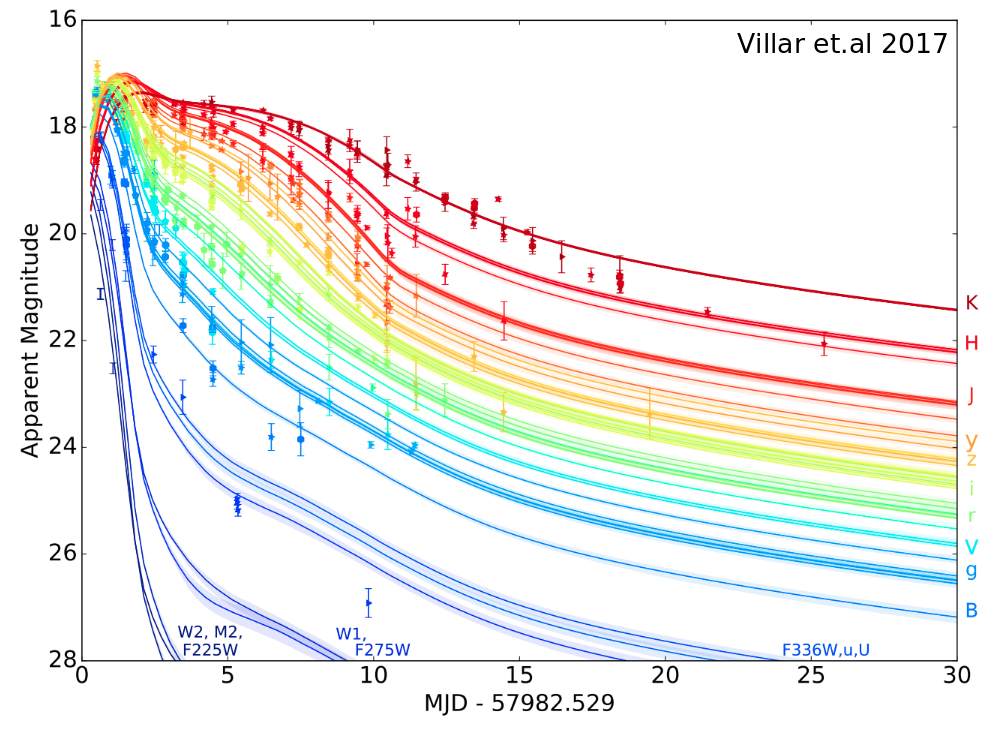
\includegraphics[height=3.8cm]{viller_mkn_model.png}
%    }};
%}
%\uncover<1->{ % <-> |
%    \node (img1) [anchor=center,scale=1,opacity=1] at ([shift={(5.5cm,-2.4cm)}]current page.center){
%        \parbox{0.5\textwidth}{
%            \includegraphics[height=3.75cm]{Ghirlanda19_afterglow.pdf}
%            %\includegraphics[height=4.0cm]{Makhathini20_grb170817_afterglow.pdf}
%    }};
%}
%
%\end{tikzpicture}
%\end{frame}
%
%
%
%
%
%
%











%\begin{frame}{}%%{Introduction}  %% ---------- Intro/motivation 
%
%\begin{tikzpicture}[overlay,remember picture]
%
%
%
%%% --------------------------------------------------------------
%
%\uncover<1->{ % <-> |
%    \node (img1) [anchor=center,scale=1,opacity=1] at ([shift={(-4.0cm,1.5cm)}]current page.center){
%        \parbox{0.5\textwidth}{
%            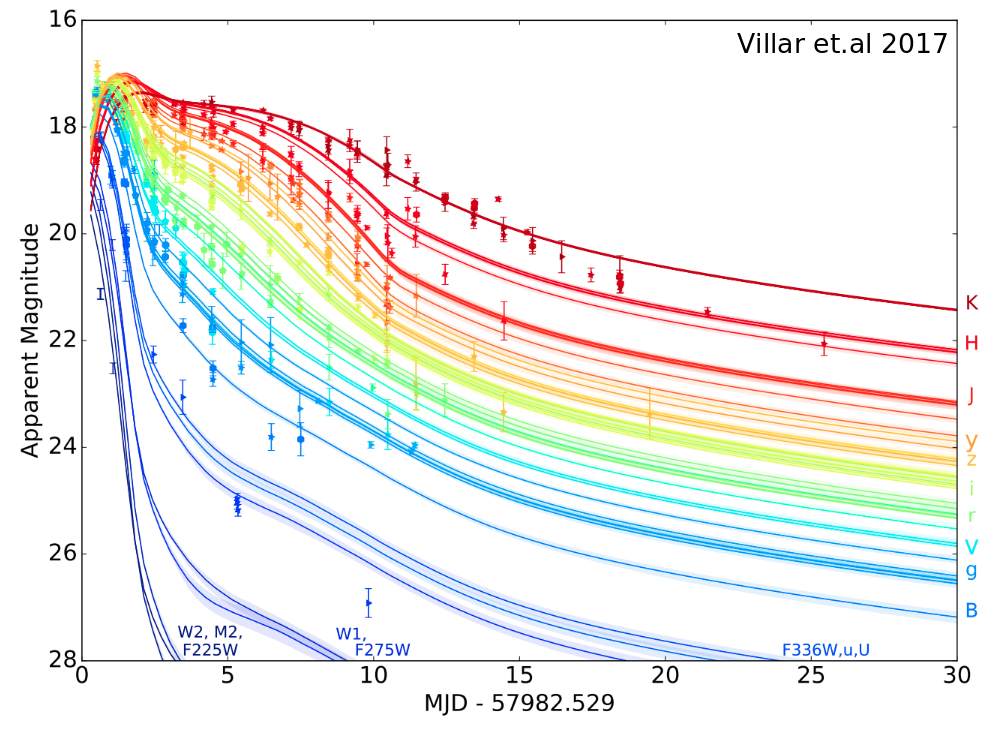
\includegraphics[height=3.8cm]{viller_mkn_model.png}
%    }};
%}
%\uncover<1->{ % <-> |
%    \node (img1) [anchor=center,scale=1,opacity=1] at ([shift={(-4.1cm,-2.4cm)}]current page.center){
%        \parbox{0.5\textwidth}{
%            \includegraphics[height=3.75cm]{Ghirlanda19_afterglow.pdf}
%            %\includegraphics[height=4.0cm]{Makhathini20_grb170817_afterglow.pdf}
%    }};
%}
%
%
%%\uncover<3->{ % <-> |
%%    \node (t1) [anchor=center,scale=1,opacity=1] at ([shift={(0.0cm,-3.8cm)}]current page.center){
%%        \parbox{0.6\textwidth}{
%%            \red{Questions}: remnant's evolution; ejecta properties; \rproc{} cites
%%    }};
%%}
%
%\uncover<1->{ % <-> |
%    \node (img1) [anchor=center,scale=1,opacity=1] at ([shift={(6.5cm,-0.0cm)}]current page.center){
%        \parbox{0.5\textwidth}{
%            \includegraphics[height=6.3cm]{jet_ascenci20.pdf}
%            
%            Artist depiction of ejecta$^\text{\citep{Ascenzi:2020xqi}}$
%    }};
%}
%
%
%\uncover<1->{ % <-> |
%    \node (img1) [anchor=center,scale=1,opacity=1] at ([shift={(1.5cm,-2.1cm)}]current page.center){
%        \parbox{0.5\textwidth}{
%            \includegraphics[height=3.5cm]{Hajela_VN_21_kn_afterglow.pdf}
%    }};
%}
%
%\end{tikzpicture}
%\end{frame}
